

\subsection{{Graphical Representation}}

	{To effectively demonstrate visually, on what the transforms and the series means and what it does to functions, we shall specifically consider the function $f(t) = e^{-t}\cdot\sin\left(2t\right)$, as this function contains both an exponential component and a sinusoidal component.}

	\subsubsection{{The Laplace Transform}}

%		\textit{}

			\begin{figure}[H]
			\centering
			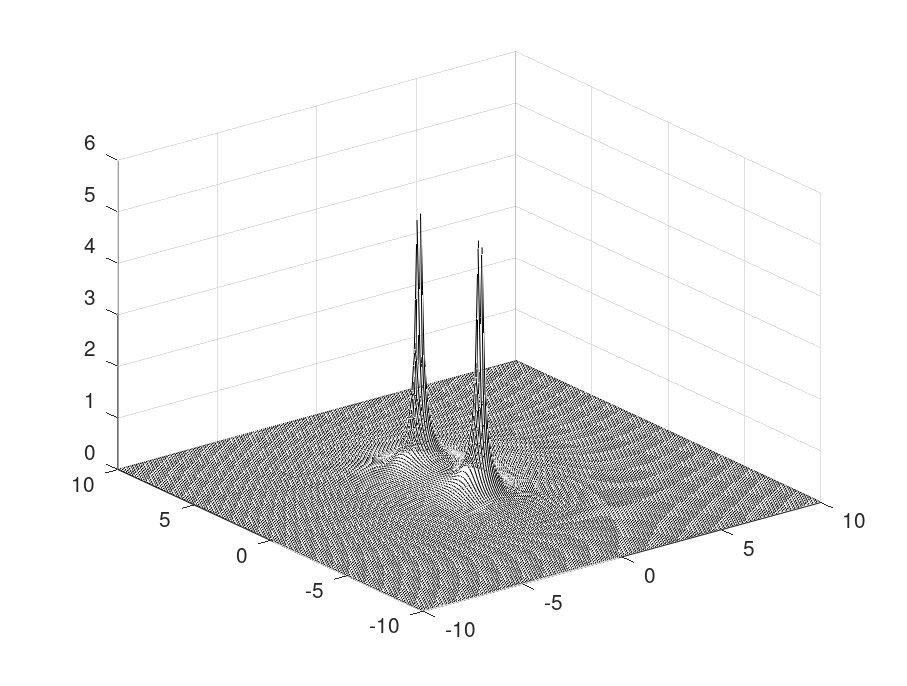
\includegraphics[width=15cm]{LapPictures/bk.png}
    		\caption{{The Laplace transform of $e^{-x}\cdot\sin\left(2x\right)$}}
			\end{figure}

		{It is evident form observing the graph of the Laplace transform of $e^{-t}\cdot\sin\left(2t\right)$, that the transform completely changes the function, all over the complex domain.}

	\subsubsection{{The Fourier Transform}}

%		\textit{}

			\begin{figure}[H]
			\centering
			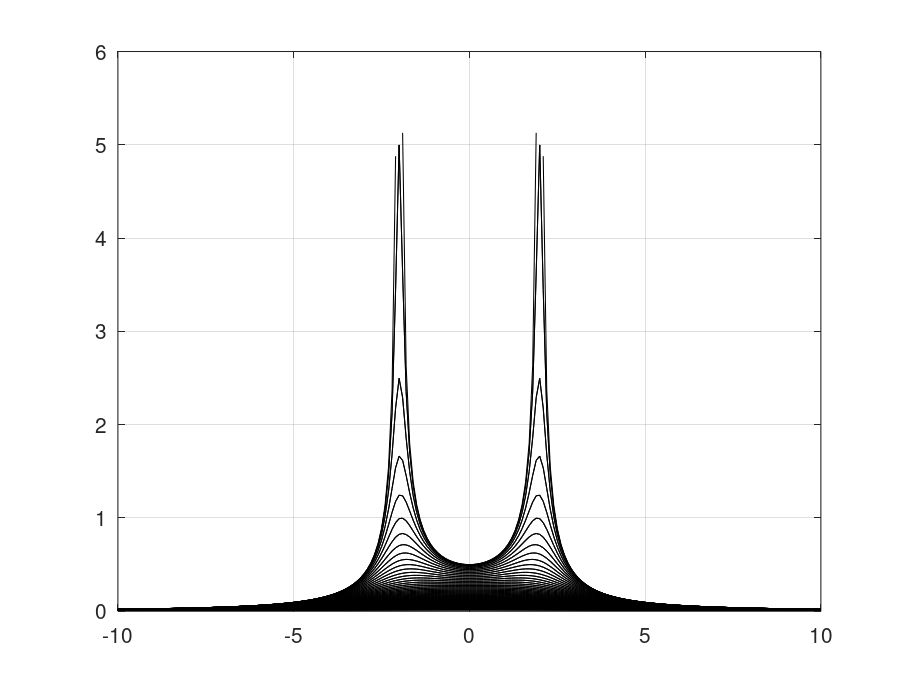
\includegraphics[width=15cm]{FouPictures/bk.png}
    		\caption{{The Fourier transform of $e^{-x}\cdot\sin\left(2x\right)$}}
			\end{figure}

		{By observation and graphical comparison, it is evident that, the Fourier transform is a slice of the Laplace transform, over the whole domain. In other words it is the Laplace transform at a specific coordinate value of the Laplace transform, ie. when the real part is zero.}

%	\subsubsection{\textit{The Fourier Series}}

%		\textit{}

%			\begin{figure}[H]
%			\centering
%			\includegraphics[width=15cm]{}
%   		\caption{\textit{The Fourier series of $e^{-x}\cdot\sin\left(2x\right)$}}
%			\end{figure}


